\documentclass[enabledeprecatedfontcommands,12pt,oneside,pdftex]{scrbook}

\usepackage{selinput}
\SelectInputMappings{
  adieresis={ä},
  germandbls={ß},
}
\usepackage[ngerman]{babel}
\usepackage{siunitx}
\usepackage{booktabs} 
\usepackage{listings}
\usepackage{color}
\usepackage{float}
\usepackage{subfigure}
\usepackage[export]{adjustbox}
\usepackage{gensymb}
\usepackage[numbers,square]{natbib}
\usepackage{amsmath}
\usepackage{tabularx}
\bibliographystyle{abbrvdin}
\usepackage{color}
\definecolor{dkgreen}{rgb}{0,0.6,0}
\definecolor{gray}{rgb}{0.5,0.5,0.5}
\definecolor{mauve}{rgb}{0.58,0,0.82}
\lstset{numbers=left,
	numberstyle=\tiny,
	numbersep=5pt,
	breaklines=true,
	showstringspaces=false,
	frame=l ,
	xleftmargin=15pt,
	xrightmargin=15pt,
	basicstyle=\ttfamily\scriptsize,
	stepnumber=1,
	keywordstyle=\color{blue},          % keyword style
  	commentstyle=\color{dkgreen},       % comment style
  	stringstyle=\color{mauve}         % string literal style
}
\lstset{language=Python}

\usepackage[automark, headsepline]{scrpage2}
% Ermöglichung von Hyperlinks (PDF-Bookmarks)
\usepackage{hyperref}

%Graphiken
\usepackage{graphicx}
\graphicspath{{Bilder/}}


\begin{document}
% ----------------------------------------------------------------------------
\titlehead{IEH - 2017}
\subject{Bericht HiWi-Tätigkeit}
\title{My Own Smarthome \\[1cm] 
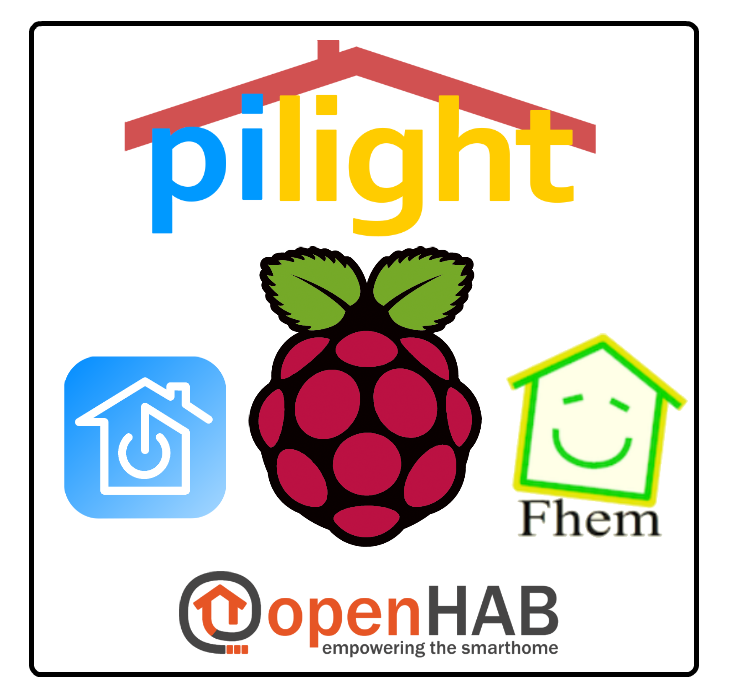
\includegraphics[width=.5\linewidth]{titelbild} 
} 
\subtitle{}
\author{Olena Manzhura, Marvin Noll}
\publishers{betreut von Sebastian Hubschneider}

\maketitle

% ----------------------------------------------------------------------------
% Inhaltsverzeichnis:
\clearpage
\pdfbookmark{\contentsname}{toc}
\tableofcontents

% ----------------------------------------------------------------------------

% Definition der Kopf- und Fußzeile
\pagestyle{scrheadings}
\ohead{\pagemark}
\chead{}
\ihead{\headmark}
\ofoot{}
\cfoot{}
\ifoot{}


\section{Auslesen der Daten von der Wetterstation}
Die Daten der Wetterstation sollen sekündlich (höchstmögliche Auflösung bedingt durch die Wetterstation) ausgelesen und in einer Datenbank gespeichert werden. Dazu wird ein Python-Skript geschrieben, welches permanent laufen soll. Den zugehörigen Quellcode zeigt Listing \ref{lst:skript}. Die einzelnen Schritte sind im Code kommentiert. Die Daten werden mit Zeitstempel in die Datenbank gespeichert. Dieser ist auch der Primärschlüssel.

\newpage

\vspace*{\fill}
\begin{figure}[H]
	\centering
	\includestandalone[width=1\textwidth]{Bilder/iehWeather}
	\caption{Flussdiagramm des Python-Skriptes zum Auslesen der Wetterdaten}
	\label{fig:logDiagram}
\end{figure}

\vspace*{\fill}

%\vspace*{\fill}
%\noindent
%\hspace*{-\oddsidemargin}

%\begin{figure}[H]
%    \centering
% \resizebox{\textwidth}{!}{\includegraphics[]{Bilder/iehWeather.tikz}}
%    \resizebox{\textwidth}{!}{\documentclass{standalone}

\begin{document}

\tikzstyle{arrow} = [thick,->,-{Latex[length=2mm, width=2mm]}]
\tikzstyle{dasharrow} = [thick,dashed,->,-{Latex[length=2mm, width=2mm]}]


%flowchart multidocument
\tikzset{
  multidocument/.style={
    shape=tape,
    draw,
    fill=white,
    tape bend top=none,
    double copy shadow},
  manual input/.style={
    shape=trapezium,
    draw,
    shape border rotate=90,
    trapezium left angle=90,
    trapezium right angle=80}}


\begin{tikzpicture}[scale=0.5]

\node (start) at (15,30) [draw, terminal,minimum width=3cm,minimum height=1cm] {START};
\node(kreis1) at (15,27) [draw, circle, minimum width=0.2 cm] {};



\node (proc1) at (15,23) [draw, process, align=left,minimum width=3cm,minimum height=2cm] {connect\\ to SQL DB};
\node (datenbank) at (5,23) [cylinder, shape border rotate=90, draw,align = left, minimum height=3cm,minimum width=3cm]
{weather \\ data};
\coordinate (point4) at (5,-5);
\node (decide1) at (15,17) [draw, decision,minimum width=2cm,minimum height=2cm] { error ?};

\node (proc2) at (27,17) [draw, process, align=left,minimum width=3cm,minimum height=1cm] {write to log\\ and increase\\ error counter};
\node (decide2) at (27,23) [draw, decision, align = left,minimum width=1cm,minimum height=1cm] {\tiny error count \\ \tiny too high ?};
\node (delay1) at (21,27) [draw, rounded rectangle, rounded rectangle east arc=0pt, minimum height = 1 cm, minimum width = 2 cm] {delay};

\node (proc7) at (37,23) [draw, process, align=left,minimum width=3cm,minimum height=2cm] {critical error; \\ send email\\ and die};
\node(log) at (37,17) [tape,tape bend top=none,draw,align = left, font=\sffamily, minimum width = 3 cm, minimum height = 2 cm]{logfile};
\coordinate (point7) at (32,16);
\coordinate (point8) at (34,16);
\node (stop) at (45,23) [draw, terminal,minimum width=3cm,minimum height=1cm] {TERMINATE};
\coordinate (point5) at (31,22);
\coordinate (point6) at (34,22);


\node (proc3) at (15,10) [draw, process, align=left,minimum width=3cm,minimum height=2cm] {determine serial\\ port of weather\\ station};
\node(kreis2) at (15,6) [draw, circle, minimum width=0.2 cm] {};
\node[circle, minimum width=3 cm] at (0,10) {};

\coordinate (point3) at (10,6);

\node (proc4) at (15,2) [draw, process, align=left,minimum width=3cm,minimum height=2cm] {read and decode\\ data from \\ weather station};

\node (proc5) at (15,-5) [draw, process, align=left,minimum width=3cm,minimum height=2cm] {write data\\ to DB};
\node (decide3) at (15,-11) [draw, decision, align = left,minimum width=2cm,minimum height=2cm] {error?};


\node (proc6) at (27,-11) [draw, process, align=left,minimum width=3cm,minimum height=2cm] {write to log \\and increase\\ error counter};
\node (decide4) at (27,2) [draw, decision, align = left,minimum width=2cm,minimum height=2cm] {\tiny error count \\ \tiny too high ?};
\coordinate (point9) at (31,2);

\node (delay2) at (21,6) [draw, rounded rectangle, rounded rectangle east arc=0pt, minimum height = 1 cm, minimum width = 2 cm] {delay};

\draw[arrow](start) -- (kreis1); 
\draw[arrow](kreis1) -- (proc1);
\draw[arrow](decide2)  |-   node[anchor=west,very near start] {no} (delay1);
\draw[arrow](delay1) -- (kreis1);
\draw[arrow](proc1) -- (decide1);
\draw[arrow](decide1) -- node[anchor=west, very near start] {no} (proc3);
\draw[arrow](decide1) -- node[anchor=north, very near start] {yes} (proc2);
\draw[arrow](proc2) -- (decide2);
\draw[arrow](proc3) -- (kreis2);
\draw[arrow](kreis2)  -- (proc4);
\draw[arrow](proc4) -- (proc5);
\draw[arrow](proc5) -- (decide3);
\draw[arrow](decide3) -| node[anchor=north, very near start] {no} (point3)--(kreis2);
\draw[arrow](decide3) -- node[anchor=north, very near start] {yes} (proc6);
\draw[arrow](proc6) -- (decide4);

\draw[arrow](delay2) -- (kreis2);
\draw[arrow] (proc7) -- (log);
\draw[arrow] (proc7) -- (stop);
\draw[arrow] (decide2) -- node[anchor=north, very near start] {yes} (proc7);
\draw[arrow] (decide4) -| node[anchor=north, very near start] {yes} (point9)--(point5)--(point6);
\draw[arrow](decide4)  |- node[anchor=west, very near start] {no} (delay2);

\draw[dasharrow] (proc5) -| node[anchor=north, near start] { write } (point4) -- (datenbank);
\draw[dasharrow] (proc1) -- node[anchor=north, midway] { connect } (datenbank);
\draw[dasharrow] (proc2) -- (log);
\draw[dasharrow] (proc6) -| (point7)--(point8);

\end{tikzpicture}
\end{document}}
%    \caption{Flussdiagramm des Python-Skriptes zum Auslesen der Wetterdaten}
%    \label{fig:test}
%\end{figure}
%\vspace*{\fill}


\newpage

\lstinputlisting[label=lst:skript,caption = {Python-Skript zum Auslesen der Daten}, language = Python]{lst/logScript.py}

\mbox

\newpage

\subsection{Scheduler}
Soll ein Stück Programmcode zyklisch aufgerufen werden, kann zum Beispiel der jeweilige Code in einer Endlosschleife platziert werden. Die gewünschte Zykluszeit $T$ kann dann näherungsweise durch Einfügen einer Wartezeit $\tau_{sleep}$ in der Schliefe erreicht werden. Kann die Ausführungsdauer des zu taktenden Programmcodes $\tau_{code}$ gegenüber $T$ vernachlässigt werden, so gilt: \begin{equation}
T\approx\tau_{sleep} \bigg\rvert_{\tau_{code} \ll \tau_{sleep}}
\end{equation}
Ist $\tau_{code}$ nicht zu vernachlässigen, ist eine genaue Taktung mit einer simplen Verzögerung nur schwer möglich, da dann die nötige Verzögerungszeit berechnet werden muss. Ist diese nicht konstant, wird die Berechnung zusätzlich erschwert.

Es bietet sich dann der Einsatz eines Schedulers an. Dieser sorgt dafür, dass eine selbst definierte Funktion in einem einstellbaren Intervall aufgerufen wird.

\subsubsection{APScheduler}
\textbf{APScheduler} (\textbf{A}dvanced \textbf{P}ython Scheduler) ist eine Python-Bibliothek, die es ermöglicht, Funktionen ("'Jobs"') zeitlich zu verwalten. Es bestehen dabei drei verschiedene Arten, dies zu tun:
\begin{enumerate}
	\item \textbf{einfache Ausführung} zu einem späteren, vorgegebenen Zeitpunkt
	\item \textbf{periodische Auführung}, bei der die Funktion in einem bestimmten Intervall wiederholt ausgeführt wird. Es besteht die Möglichkeit, zudem einen Start- und Endzeitpunkt anzugeben.
	\item "'\textbf{cron-style}"'- Ausführung, bei der die Funktion zu einer bestimmten Uhrzeit ausgeführt wird. Auch hier besteht die Möglichkeit, einen Start- und Endzeitpunkt anzugeben. Diese Funktionsweise ähnelt dem "'Cron-Daemon"' in Linux bzw. anderen unixartigen Betriebssystemen.
\end{enumerate}

\paragraph{Installation}

Eine beliebige Version wird mit folgender Zeile installiert (für "'x.x.x"' die gewünschte Version eintragen):\\ \texttt{sudo pip3 install apscheduler==x.x.x}. \\
Für Python 3 benötigt man die aktuelle Version 3.3.1 (Stand Oktober 2017).

\paragraph{Beispiel für eine periodische Ausführung}

Ein Beispiel für das periodische Ausführen einer Funktion ist in Listing \ref{lst:apbeispiel} aufgeführt.\\
Zunächst wird die Funktion, die periodisch ausgeführt werden soll definiert (im Beispiel ist das "'job\_function"'). Anschließend wird je nach Situation der entsprechende Scheduler ausgewählt. Im Beispiel wird der "'BackgroundScheduler"' gewählt, welcher eingesetzt wird, wenn einzig der Scheduler laufen soll. Weitere Arten können in der Dokumentation zum APScheduler nachgeschaut werden. \\
Zum Schluss wird die vorher definierte Funktion dem Scheduler zugewiesen, der sie jede Sekunde ausführt.

\lstinputlisting[label=lst:apbeispiel,caption = {Beispiel für periodische Ausführung}]{lst/periodAusf.py}


\paragraph{Umsetzung beim Wetterdaten-Skript}

\autoref{lst:apWetterdaten} zeigt das mit APScheduler realisierte Wetterdaten-Skript. Im Gegensatz zur Realisierung mit der "'\textbf{sleep}"'-Funktion wird das Auslesen der Daten jetzt nur \textbf{alle zwei Sekunden} ausgeführt. Dies liegt daran, dass die Ausführung des gesamten Codes etwas länger dauert. Es entsteht ein Konflikt, da die nächste Funktion aufgerufen wird, bevor die vorherigeabgeschlossen ist. Für Darstellungszwecke wurden Code-Abschnitte, die schon aus anderen Kapiteln bekannt sind, ausgelassen.

\lstinputlisting[label=lst:apWetterdaten,caption = {Wetterdaten-Skript mit APScheduler}]{lst/apScheduler.py}

\newpage

\subsection{SQL Datenbank}

\subsubsection{Verschieben der Datenbank auf externes USB-Laufwerk}
Da der Raspberry Pi selbst nicht sehr viel Speicher besitzt, kann es sinnvoll sein, das Datenbank-Verzeichnis bzw. die zu speichernden Daten auf ein externes Laufwerk mit mehr Speicherkapazität zu verschieben.\\
Normalerweise bindet Raspbian Jessie angeschlossene USB-Laufwerke \textbf{automatisch} im Pfad \texttt{/media/\{USERNAME\}/\{LABEL\}} ein. Dies geschieht aber nur, wenn der Benutzer angemeldet ist.\\
Zum automatischen Einbinden (auch ohne Anmeldung) kann der Befehl \texttt{usbmount} genutzt werden. Allerdings besteht hier das Problem, dass man nicht sicher sein kann, unter welchem Verzeichnis das Laufwerk eingebunden wird und müsste dieses somit jedes Mal im Dateisystem suchen. Dieser Ansatz ist deshalb für Datenbank-Zwecke nicht geeignet.\\
Im Folgenden werden die Schritte beschrieben, die benötigt werden, um eine Festplatte/einen USB-Stick einzubinden und einem festen Verzeichnis zuzuordnen.

\paragraph{Einbinden des externen Laufwerks}

\begin{enumerate}
	\item \textbf{Überprüfen, welche Dateisysteme unterstützt werden: } \\
	Damit das Dateisystem auf dem Laufwerk erkannt wird, muss das entsprechende Dateisystem-Modul installiert sein. Die vorhandenen Module können mit dem Befehl \texttt{ls -1 /lib/modules/\$(uname -r)/kernel/fs} aufgelistet werden.\\
	Für NTFS-Partitionen wird das Paket \texttt{ntfs-3g} benötigt. Dieses sollte bei \textbf{Raspbian Jessie} automatisch installiert werden.
	\item \textbf{Laufwerk identifizieren: } \\
	Durch Aushängen des Laufwerks und anschließendes Einhängen in Kombination mit den Befehlen \texttt{lsblk} und \texttt{df -h} kann die Festplatte/der USB-Stick identifiziert werden.
	Diese werden in der Regel mit "'\textbf{sda}"' , "'\textbf{sdb}"', usw. angezeigt. Die darauf befindlichen Partitionen werden mit "'\textbf{sda1}"', "'\textbf{sda2}"', ... bezeichnet.
	\item \textbf{Bestimmen der UUID\footnote{\textbf{U}niversally \textbf{U}nique \textbf{Id}entifier - eindeutig für jedes Gerät bestimmt, solange es nicht formatiert wird}: }\\
	Für das automatische Einbinden des Laufwerks nach Neustart des Systems wird die UUID des Gerätes benötigt. Mit \texttt{sudo blkid} wird die UUID, zusammen mit anderen Informationen, für jedes angeschlossene Gerät aufgelistet.
	\item{\textbf{Laufwerk fest einem Mount-Point zuordnen: }\\
		Mit \texttt{/etc/fstab} öffnet man die Datei \textbf{fstab}. In ihr sind die Dateisysteme eingetragen, mit denen die Partitionen auf dem Laufwerk formatiert sind. 
		Das Laufwerk sollte in folgender Form eingetragen werden: \\
		\texttt{\small UUID=uuid mountpoint dateisystem auto,nofail,sync,users,rw,umask=000   0   0
		}\\
		Statt "'uuid"' wird die jeweilige UUID des Laufwerks eingetragen.
		"'mountpoint"' bezeichnet das Verzeichnis, an das später das Laufwerk gebunden werden soll (z.B. \texttt{/media/usb}). Die beim Laufwerk verwendete Formatierung wird statt "'dateisystem"' eingetragen (z.B. "'vfat"' für Dateisysteme, die mit "'FAT"' formatiert wurden). Die restlichen Optionen können bei Bedarf unter \cite{c6} nachgeschaut werden.}
	
	\item{\textbf{Erstellen des Verzeichnisses für den Mount-Point: }\\
		Dies geschieht mit \texttt{sudo mkdir -p verzeichnispfad} (für obiges Beispiel \texttt{sudo mkdir -p /media/usb}). Anschließend wird das Laufwerk manuell eingehängt:  \texttt{sudo mount -a}.\\
		Mit \texttt{df -h} und \texttt{lsblk} prüft man, ob das Laufwerk in das Verzeichnis eingehängt wurde, das in "'fstab"' angegeben wurde.
		
	} 
\end{enumerate}

\subsubsection{Abschätzung benötigter Speicherplatz}

\subsubsection{Verschieben des Datenbank-Verzeichnisses auf das Laufwerk}


\subsubsection{Fernzugriff auf die Datenbank}
In der Standardkonfiguration eines MySQL-Servers ist der Zugriff auf die Datenbanken des Servers von außen aus Sicherheitsgründen gesperrt. Das bedeutet, der Zugriff auf die Daten ist nur indirekt z.B. über eine php-Seite möglich. Ist es hingegen gewünscht direkt auf den SQL-Server zuzugreifen, zum Beispiel über eine direkte TCP-Verbindung, oder eine Abstraktionsebene, wie ODBC\footnote{\textbf{O}pen \textbf{D}ata\textbf{b}ase \textbf{C}onnectivity}, dann muss der mySQL-Server dafür explizit konfiguriert werden. (Stand Juni 2017, mySQL-Version 5.17.18)
Dazu werden folgende Schritte durchgeführt:

\begin{enumerate}
	\item In der Konfigurationsdatei \texttt{my.cnf} im Verzeichnis \texttt{/etc/mysql/} wird der Wert von \texttt{bind-address} (Standardwert \texttt{127.0.0.1}) auf \texttt{0.0.0.0} geändert. Dadurch werden Verbindungen von einer beliebigen IP-Adresse statt nur dem lokalen Computer erlaubt.
	\item Es wird sichergestellt, dass der gewünschte Datenbankuser seine zugeteilten Rechte von jedem beliebigen Host aus ausüben kann. Dazu wird z.B. mit phpMyAdmin die Benutzerverwaltung geöffnet. Darin muss in der Spalte \texttt{host} des entsprechenden Benutzers der Wert \texttt{\%} eingetragen sein. Alternativ kann dies über das SQL-Kommando\footnote{SQL-Kommandos können zum Beispiel über phpMyAdmin \texttt{Server -> SQL} an den Server gesendet werden}
	\begin{verbatim}
	GRANT ALL PRIVILEGES ON *.* TO 'db_user'@'%'
	IDENTIFIED BY '1234'
	WITH GRANT OPTION;
	FLUSH PRIVILEGES;
	\end{verbatim}
	erreicht werden. Dabei ist \texttt{db\_user} der Benutzer mit dem Passwort \texttt{1234} und bekommt alle Rechte auf dem Server(Aus offensichtlichen Gründen nur für Testzwecke empfohlen).
\end{enumerate}


\paragraph{Unmount}
http://ramiro.org/blog/usbdrive-unter-linux-formatieren/


\subsubsection{Datenbankzugriff mit ODBC}
Mit Hilfe eines ODBC(\textbf{O}pen \textbf{D}ata\textbf{b}ase \textbf{C}onnectivity) Connectors ist ein einfacher Zugriff auf viele Datenbanken möglich. Der Vorteil in der Benutzung eines ODBC-Connectors liegt darin, dass durch den Connector die Kommunikation mit der Datenquelle soweit abstrahiert wird, dass ein einfacher Zugriff auf die Daten möglich wird, ohne auf die Datenquelle direkt zugreifen zu müssen. Dadurch werden Programmierfehler vermieden und der Typ der Datenquelle spielt nur noch eine untergeordnete Rolle. Prinzipiell kann die MySQL-Datenbank so beispielsweise durch eine PostgreSQL oder eine MS-Access-Datenbank ersetzt werden, ohne dass Änderungen am Programmcode nötig wären.
Nachteilig ist, dass es für die Zielplattform einen ODBC-Treiber für die jeweilige Datenbankanwendung geben muss. Für Windows und gängige Linux-Distributionen ist dies jedoch meistens der Fall.

\paragraph{Installation des MySQL ODBC-Treibers unter Windows}

Für die Nutzung des ODBC-Connectors für mySQL unter Windows (x86 und x64) sind die folgenden Schritte erforderlich:
\begin{enumerate}
	\item Download des ODBC-Treibers (unter: \texttt{https://dev.mysql.com/downloads/\\connector/odbc/}). Dabei ist zu beachten, dass 32-bit Anwendungen den 32-bit Treiber und 64-bit Anwendungen den 64-Bit Treiber benötigen.
	\item Installation des heruntergeladenen Treibers
	\item Öffnen des Datenquellenadministrationstools:
	\begin{itemize}
		\item 32-Bit: \texttt{C:\textbackslash Windows\textbackslash SysWOW64\textbackslash odbcad32.exe}
		\item 64-bit: \texttt{C:\textbackslash Windows\textbackslash System32\textbackslash odbcad32.exe}
	\end{itemize}
	\item \texttt{User DSN -> Add...}
	\item \texttt{'MySQL ODBC x.x Unicode Driver' -> Finish}
	\item Parameter der Verbindung eingeben:
	\begin{itemize}
		\item \texttt{Data Source Name}: beliebiger Name
		\item \texttt{TCP/IP Server}: IP-Adresse des mySQL-Servers 
		\item \texttt{User}: Benutzer (mit passenden Rechten)
		\item \texttt{Password}: Passwort des Benutzers
		\item \texttt{Database}: gewünschte Datenbank auswählen
	\end{itemize}
	\item \texttt{Ok}
\end{enumerate}


\newpage

%\subsection{WAMP}

%\lstinputlisting[caption = {wampThiesWetterstationToESHLWamp}, language = Python]{thiesToWAMP.py}


%\lstinputlisting[caption = {wampWetterstationSubscriber}, language = Python]{wetterstationSubs.py}

%\newpage



\subsection{Python Skripte für die Wetterstation als Daemon(Systemdienst)}
\subsubsection{Motivation}
Wenn ein Programm als Dienst/Hintergrundprogramm/Daemon dauerhaft ausgeführt werden soll, sollten die folgenden Fragen geklärt werden:
\begin{itemize}
	\item Wann und von wem wird der Dienst gestartet?
	\item Wann und von wem wird der Dienst beendet?
	\item Was passiert, wenn ein Laufzeitfehler auftritt?
	\item Was passiert, wenn das Dienstprogramm unerwartet abstürzt?
\end{itemize}

Für Testzwecke ist es meist ausreichend, das Programm von Hand zu starten und gelegentlich manuell zu prüfen, ob Fehler aufgetreten sind. Ist die Entwicklung des Programms abgeschlossen, ist es zweckmäßig es vom System als Dienst starten zu lassen. Dienste, wie \textit{SystemVinit} oder das modernere \textit{systemd} ermöglichen es, Programme automatisch zu starten, bei Bedarf zu beenden und zu überwachen.

\subsubsection{Minimalbeispiel Daemon mit \textit{systemd}}
In diesem Abschnitt wird anhand eines Beispiels demonstriert, wie mit Hilfe von \textit{systemd} ein eigener Dienst erstellt wird. Dazu ist eine ausführbare, nicht interaktive\footnote{d.h. das Programm muss ohne Benutzerinteraktion lauffähig sein, darf also keine GUI oder Konsoleninteraktion enthalten. Laufzeitfehler sollten, wenn möglich, abgefangen werden.} Programmdatei nötig.

Die folgenden Schritte sorgen dafür, dass die Datei \texttt{test.py} beim Systemstart von systemd automatisch gestartet wird. Beim Herunterfahren des Systems wird das Programm lediglich abgebrochen. Die Vorgehensweise ist unter \textit{raspberrypi 4.9.80-v7+} getestet.

\begin{enumerate}
	\item im Ordner \texttt{/etc} wird mit root-Rechten ein neuer Ordner für den Dienst angelegt:
	\begin{lstlisting}
	$ sudo mkdir /etc/test
	\end{lstlisting}
	
	\item Die ausführbare Programmdatei(In diesem Beispiel "'test.py"', bestehend aus einer Endlosschleife mit einer Verzögerung) wird in den neu erstellten Ordner verschoben:
	\begin{lstlisting}
	$ sudo mv test.py /etc/test/test.py
	\end{lstlisting}
	
	\item Der Besitzer der Datei sollte root sein und die Datei muss ausführbar sein. Der Erfolg der Operationen wird anschließend mit \texttt{ls -l} überprüft:
	\begin{lstlisting}
	$ cd /etc/test
	$ sudo chown root test.py
	$ sudo chmod 755 test.py
	$ ls -l
	-rwxrwxr-x 1 root root 2638 Jun 20 20:45 test.py
	\end{lstlisting}
	
	\item Es wird überprüft, ob das Programm als root ausgeführt werden kann. Insbesondere mit \textit{pip} installierte Zusatzpakete können zu Problemen führen, da diese i.d.R. nur für die aktuellen Benutzer installiert werden.
	\begin{lstlisting}
	$ sudo python3 /etc/test/test.py
	
	\end{lstlisting}
	
	\item Für den Dienst wird eine \texttt{*.service} Konfigurationsdatei benötigt. Diese wird im Verzeichnis \texttt{/etc/systemd/system} angelegt:
	
	\lstinputlisting[label=lst:service,caption = {Beispiel für eine Service-Konfigurationsdatei}]{lst/service.txt}
	
	Wichtig ist, dass unter \texttt{ExecStart} der \textbf{absolute} Pfad zum Interpreter anzugeben ist. Im Beispiel würde also \texttt{python3 /etc/test/test.py} nicht funktionieren.
	
	\item Damit der neu erstellte Dienst systemd bekannt wird und automatisch gestartet wird, wird \textit{systemctl} verwendet. Ob der Dienst erfolgreich gestartet werden konnte, wird \texttt{systemctl status} überprüft.
	\begin{lstlisting}
	$ sudo systemctl daemon-reload
	$ sudo systemctl enable test.service
	$ systemctl status test.service
	o test.service - test Daemon
	Loaded: loaded (/etc/systemd/system/test.service; enabled; vendor preset: enabled)
	Active: active (running) since Wed 2018-06-20 20:46:26 CEST; 3 weeks 3 days ago
	Main PID: 4282 (python3)
	CGroup: /system.slice/test.service
	|-4282 /usr/bin/python3 /etc/test/test.py
	
	Jun 20 20:46:26 raspberrypi systemd[1]: Started test Daemon.
	\end{lstlisting}
	
	\item Nach einem Neustart(\texttt{sudo restart}) sollte der Dienst automatisch gestartet werden.
	
	\item Dienste können mit systemctl gestoppt(\texttt{systemctl stop test.service}), neu gestartet(\texttt{systemctl restart test.service}) oder deaktiviert(\texttt{systemctl disable test.service}) werden.
\end{enumerate}

\newpage

\subsection{Starten der Wetterstationssoftware als Daemon}
Für die Software der Wetterstation werden, gemäß der Unix Philosophie \textit{"'Make each program do one thing well. To do a new job, build afresh rather than complicate old programs by adding new "'features"'"'}, zwei Dienste angelegt:
\begin{itemize}
	\item \textbf{ieh\_WetterLogd:} Schreibt die Live-Wetterdaten kontinuierlich in die Datenbank
	\item \textbf{ieh\_WetterAveraged:} Bildet über mehrere festgelegte Intervalle Mittelwerte der Wetterdaten und schreibt diese in die Datenbank.
\end{itemize}

Dazu wird, wie oben beschrieben, vorgegangen. Das Ergebnis:
\begin{lstlisting}
pi@raspberrypi:/etc/iehWetter $ cd /etc/iehWetter/
pi@raspberrypi:/etc/iehWetter $ ls -l
total 20
-rwxr-xr-x 1 root root 5116 Jul 15 12:37 wetterAveraged.py
-rwxrwxr-x 1 root root 2638 Jun 20 20:45 wetterLogd.py
pi@raspberrypi:/etc/iehWetter $ cd /etc/systemd/system/
pi@raspberrypi:/etc/systemd/system $ ls -l | grep ieh
-rw-r--r-- 1 root root  285 Jul 15 12:47 ieh_wetterAverage.service
-rw-r--r-- 1 root root  321 Jun 20 20:46 ieh_wetterLog.service
pi@raspberrypi:/etc/systemd/system $ systemctl status ieh_wetterLog.service 
o ieh_wetterLog.service - IEH wetter logger daemon for DLXmet weather station over RS232
Loaded: loaded (/etc/systemd/system/ieh_wetterLog.service; enabled; vendor preset: enabled)
Active: active (running) since Wed 2018-06-20 20:46:26 CEST; 3 weeks 3 days ago
Main PID: 4282 (python3)
CGroup: /system.slice/ieh_wetterLog.service
|-4282 /usr/bin/python3 /etc/iehWetter/wetterLogd.py

Jun 20 20:46:26 raspberrypi systemd[1]: Started IEH wetter logger daemon for DLXmet weather station over RS232.
pi@raspberrypi:/etc/systemd/system $ systemctl status ieh_wetterAverage.service 
o ieh_wetterAverage.service - IEH wetter averager
Loaded: loaded (/etc/systemd/system/ieh_wetterAverage.service; enabled; vendor preset: enabled)
Active: active (running) since Sun 2018-07-15 12:58:54 CEST; 3h 32min ago
Main PID: 13412 (python3)
CGroup: /system.slice/ieh_wetterAverage.service
|-13412 /usr/bin/python3 /etc/iehWetter/wetterAveraged.py

Jul 15 12:58:54 raspberrypi systemd[1]: Started IEH wetter averager.
\end{lstlisting}



\subsection{Überwachung der Systemauslastung mit \textit{sa}}

%TODO:
\begin{itemize}
	\item einrichtung sysstat
	\item sar
	\item isag o.Ä.
\end{itemize}












\section{OpenHAB}
"'\textbf{OpenHAB}"'\footnote{\textbf{open} \textbf{H}ome \textbf{A}utomation \textbf{B}us} ist eine Software, die Komponenten für die Hausautomation verschiedenster Hersteller auf einer Plattform vereint. Als UI werden Webbrowser, Android- oder iOS-Systeme unterstützt. Die aktuelle Version ist OpenHAB 2 (Stand: 19.07.2017). \newline

\subsection{Installation auf Linux (Raspbian Jessie)}

\begin{enumerate}
	\item Schlüssel für Bintray Paketquelle hinzufügen \newline
	\texttt{wget -qO - 'https://bintray.com/user/downloadSubjectPublicKey?username=\\openhab' | sudo apt-key add -}
	
	\item Apt erlauben, das HTTPS-Protokoll zu nutzen\newline
	\texttt{sudo apt-get install apt-transport-https}
	
	\item OpenHAB 2 Paketquelle (stabile Version) in die Quellenliste kopieren\newline
	\texttt{echo 'deb https://dl.bintray.com/openhab/apt-repo2 stable main' | sudo tee /etc/apt/sources.list.d/openhab2.list}
	
	\item Paketindex erneuern\newline
	\texttt{sudo apt-get update}
	
	\item OpenHAB 2 installieren\newline
	\texttt{sudo apt-get install openhab2}
	
	\item \textbf{Optional}: Um die Komponenten für die Hausautomatisierung zu steuern, werden bei OpenHAB Add-Ons bzw. Bindings installiert. Diese werden üblicherweise aus dem Internet heruntergeladen. Möchte man jedoch auch offline Add-Ons installieren können, besteht die Möglichkeit, das Add-Ons-Package zu installieren, sodass man auch ohne Internet zusätzliche Module installieren kann. Dies geschieht mit : \texttt{sudo apt-get install openhab2-addons} \cite{c2}
	
	\item OpenHAB 2 starten (das erste Starten kann bis zu 15 Minuten dauern)
	
	\texttt{sudo systemctl start openhab2.service}\newline
	\texttt{sudo systemctl daemon-reload}\newline
	\texttt{sudo systemctl enable openhab2.service}\newline
	
	Abfragen des Status:\newline
	\texttt{sudo systemctl status openhab2.service}
	
\end{enumerate}

\newpage

\textbf{Konfiguration}

Nach der Installation sollte unter \texttt{https://localhost:8080} (\texttt{https://ipadressedes-\\openhabservers:8080}) das OpenHAB2-Portal (s. Abb. \ref{fig:ohportal}) erreichbar sein.

\begin{figure}[H]
	\centering
	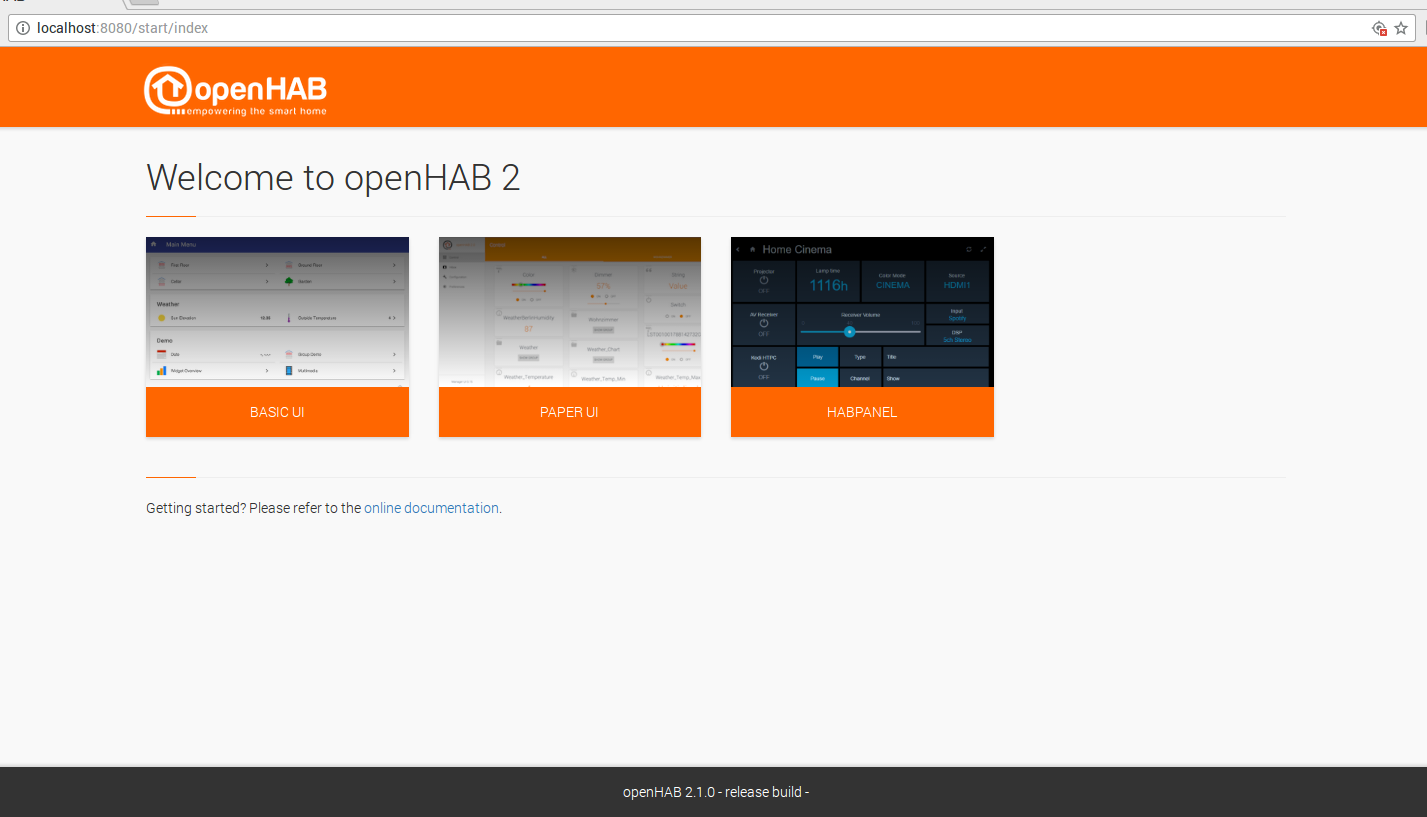
\includegraphics[width=1\textwidth]{Bilder/ohPortal}
	\caption{OpenHAB2-Portal}
	\label{fig:ohportal}
\end{figure}

Dort kann man zwischen drei verschiedenen Oberflächen wählen. Das "'\textbf{Basic UI}"' und "'\textbf{HAB Panel}"' werden dabei rein für die Darstellung und Steuerung der verschiedenen Komponenten des Smarthomes genutzt.

Zur Konfiguration von OpenHAB wird das "'\textbf{Paper UI}"' genutzt.
Dort können unter der Option "'\textbf{Add-Ons}"' unter "'\textbf{Bindings}"' neue Module installiert werden. Sie stellen die Schnittstelle zwischen dem Programm und der Hardware bzw. den Smart-Home-Komponenten dar.\newline


\subsection{Items}
Items sind die Grund-Datentypen in OpenHAB. Mit ihnen lassen sich die Komponenten des Smarthomes steuern. So kann man mit einem Item des Typs "'Switch"' schaltbare Steckdosen, Relais, etc. schalten. Alle möglichen Typen sind in \autoref{tbl:items} aufgeführt.

\begin{table}[H]
	\centering
	\setlength\extrarowheight{2pt}
	\begin{tabularx}{\textwidth}{LXX}  
		\toprule
		\textbf{Typ} & \textbf{Beschreibung} & \textbf{Mögliche Befehle}\\
		\midrule
		Color 	&  Speichert Farbinformation (RGB) &   OnOff, IncreaseDecrease, Percent, HSB 	\\
		Contact	&  Speichert Status von elektrischen Kontakten. Enthält nur Statusinformation, keine Befehle möglich. &	OpenClosed    \\
		DateTime   &	Speichert Datum und Uhrzeit & - \\
		Dimmer   & Wert für Dimmern (in Prozent) & OnOff, IncreaseDecrease, Percent\\
		Group   & Gruppiert mehrere Items zu einem Item. & -\\
		Image   & Binärdaten eines Bildes & -\\
		Location   & GPS Koordinaten & Point\\
		Number   & Zahlenwert & Decimal\\
		Player  & Kontrolle über Player (z.B. Audio-Player) & PlayPause, NextPrevious, RewindFastforward\\
		Rollershutter & Kontrolle über Rolladen& UpDown, StopMove, Percent\\
		String & Speichert Text & String \\
		Switch & An/Aus-Schalter& OnOff\\
		\bottomrule 
	\end{tabularx}
	\caption{Item-Datentypen und jeweils möglichen Befehlen}
	\label{tbl:items}
\end{table}

\subsection{Things}
\subsection{Sitemap}

\begin{table}[H]
	\centering
	\setlength\extrarowheight{2pt}
	\begin{tabularx}{\textwidth}{LX}  
		\toprule
		\textbf{Element} & \textbf{Beschreibung}\\
		\midrule
		Chart 	&  Diagramm\\
		Colorpicker	&  Farbauswahl \\
		Default   &	Rendert ein Objekt abhängig vom Itemtyp \\
		Frame   & Gruppierung/Umrahmung mehrerer Sitemap-Elemente. \\
		Group   & Gruppiert die angegebenen Elemente in einen Block.\\
		Image   & Bild (gegeben durch URL)\\
		Mapview   & OSM Karte \\
		Selection   & Dropdown Menü um ein Item auszuwählen \\
		Setpoint  & Wert mithilfe +/- Buttons auswählen \\
		Slider & Schieberegler \\
		Switch & An/Aus-Schalter \\
		Text & Beschriftung \\
		Video & Zeigt ein Video (angegeben durch URL) \\
		Webview & Zeigt Inhalt einer Webseite.\\
		\bottomrule 
	\end{tabularx}
	\caption{Sitemap-Typen}
	\label{tbl:sitemapss}
\end{table}



\subsection{OpenHAB Android-App}
Die OpenHAB App ist für Android und iOS verfügbar und bietet die Möglichkeit, den OpenHAB-Server bzw. OpenHAB-Cloud-Instanzen (s. \autoref{fig:ohCloud}) zu steuern.

Die App verbindet sich entweder über die lokale Server-URL (bzw. IP-Adresse) mit dem Openhab-Dashboard oder über Fernzugriff mit \texttt{https://myopenhab.org}. Hierfür muss man einen Account bei \texttt{myopenhab.org} anlegen und die Anmeldeinformationen in den Einstellungen der App eingeben.

Seitens OpenHAB muss der \textit{OpenHAB Cloud Connector} eingebunden werden und die URL für den OpenHAB Cloud Server eingegeben werden (\texttt{https://myopenhab.org}).


\paragraph{Anmerkung zur Registrierung bei myopenhab.org}

Zur Registrierung bei myopenhab.org sind unter Anderem die \textit{openHAB UUID} und das \textit{openHAB Secret} notwendig. Ersteres lässt sich mit \texttt{cat /var/lib/openhab2/uuid}, das Secret mit \texttt{cat /var/lib/openhab2/openhabcloud/secret} ausgeben.


\begin{figure}[H]
	\centering
	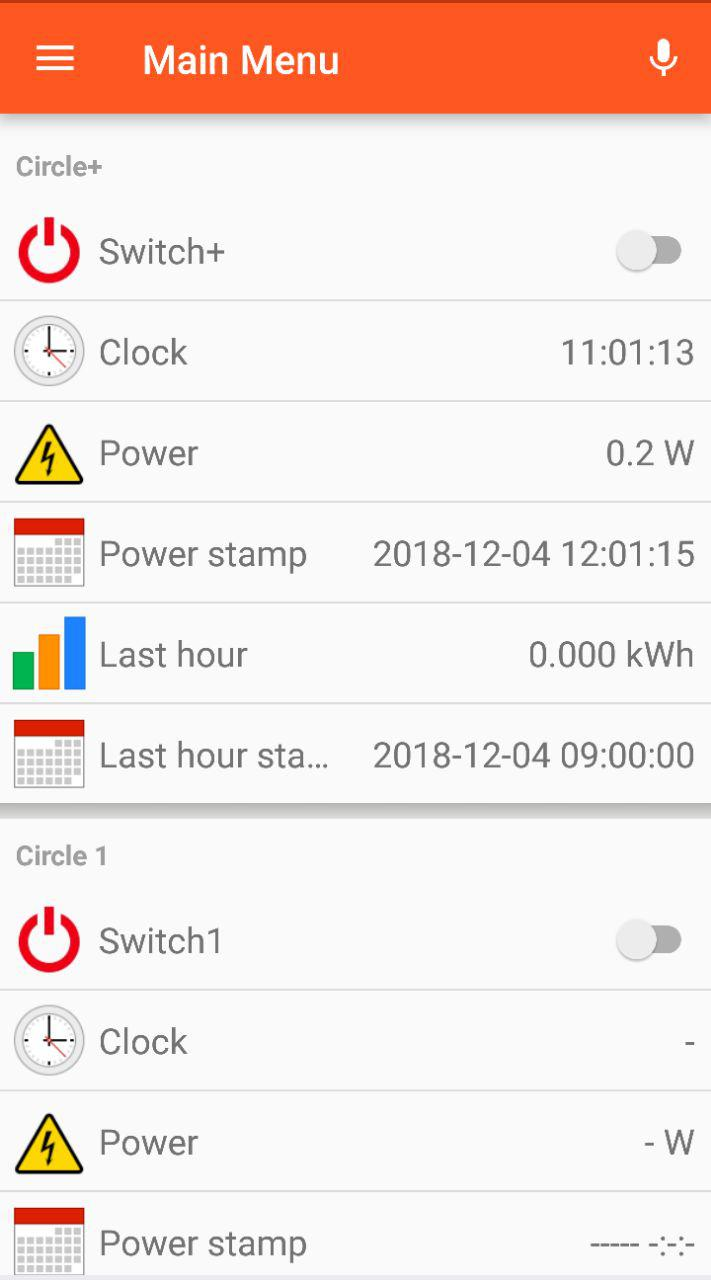
\includegraphics[width=0.3\textwidth]{Bilder/App}
	\caption{Benutzeroberfläche der OpenHAB Android App}
	\label{fig:ohCloud}
\end{figure}

\begin{figure}[H]
	\centering
	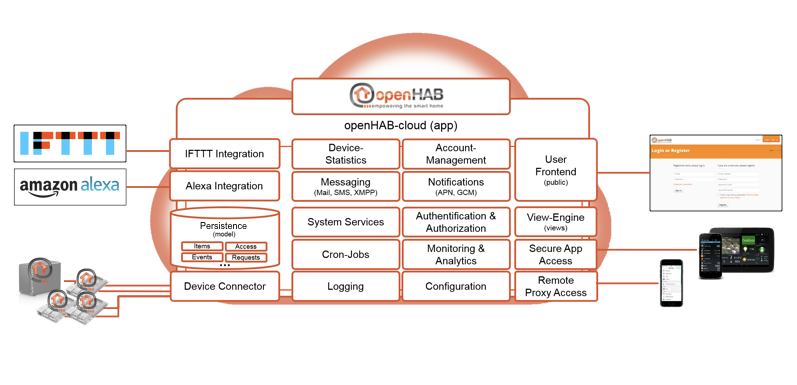
\includegraphics[width=0.9\textwidth]{Bilder/openHAB-Cloud}
	\caption{Architektur der OpenHAB-Cloud}
	\label{fig:ohApp}
\end{figure}

\newpage


\section{Schaltbare Steckdosen}
\subsection{Steckdosen von Plugwise}

Das vorhandene Set besteht aus 6 Steckdosen und einem USB-Stick zur Kommunikation mit einem Rechner. Die Steckdosen bieten neben der Möglichkeit des Ein- und Ausschaltens auch die Aufzeichnung des Stromverbrauches eines angeschlossenen Gerätes. 

\begin{figure}[h!]
	\centering
	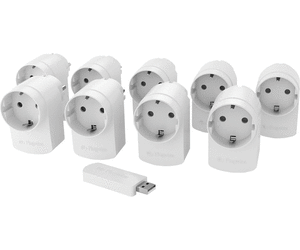
\includegraphics[width=6cm]{Bilder/pwsteckdosen.png}
	\caption{Plugwise Steckdosen mit Stick}
\end{figure}

\subsubsection{Kommunikation und Netzwerkaufbau} 

Die Steckdosen, auch "'\textbf{Circles}"' oder Module genannt, kommunizieren untereinander über das \textbf{ZigBee}-Protokoll\footnote{'ZigBee ist eine Spezifikation für drahtlose Netzwerke mit geringem Datenaufkommen, wie beispielsweise Hausautomation, Sensornetzwerke, Lichttechnik' \cite{c1}} %fußnote einfügen. \\
Die einzelnen Module werden zu einem Netzwerk zusammengefügt. Dies geschieht üblicherweise mittels der herstellereigenen Software "'\textbf{Plugwise Source}"' (nur für Windows verfügbar). Die Konfiguration des Netzwerks geschieht über das "'\textbf{Circle+}"' und den "'\textbf{Plugwise-Stick}"'. Letzterer dient als Schnittstelle zwischen Computer und Steckdosen. Das \textbf{Circle+} speichert alle dem jeweiligen Netzwerk angehörigen \textbf{Circles}, ansonsten fungiert es als gewöhnliche Funksteckdose. \newline
Die Übertragung der Daten (Status,Stromverbrauch,...) findet über Wege von Modul zu Modul statt,sodass auch weiter entfernte Geräte angesprochen werden können.\\
Zugriff auf die Module anderer Netzwerke ist mit Hilfe von zusätzlicher Hardware \\ (\textbf{Plugwise Stretch Lite}) möglich. \newline
Ein Netzwerk sollte immer so aufgebaut sein, dass \textbf{Plugwise-Stick} und \textbf{Circle+} direkten "'Sichtkontakt"' haben und jede Steckdose immer jeweils eine anderes Modul hat, an das sie Daten weiterschicken kann. Im Optimalfall (optimale Datengeschwindigkeit) ist das Netzwerk wie in Abb. \ref{fig:netzwerk} rechts angeordnet, wobei sich der \textbf{Plugwise-Stick} zudem möglichst zentral befindet.
% bild plugwise-netzwerk einfügen

%TODO Abbildung schöner zeichnen
\begin{figure}[H]
	\centering
	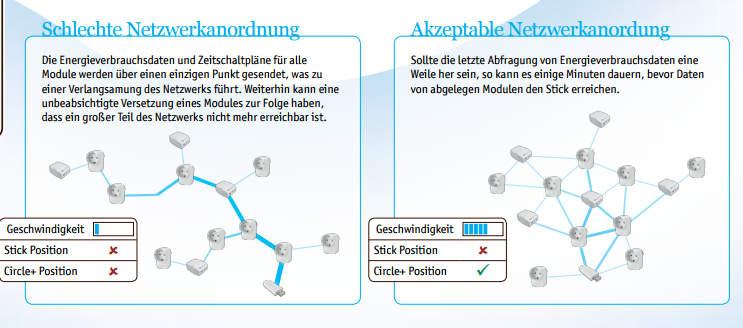
\includegraphics[width=1\textwidth]{Bilder/plugwise-netzwerk}
	\caption{Plugwise-Netzwerk}
	\label{fig:netzwerk}
\end{figure} \mbox{}

\subsubsection{Möglichkeiten zum Ansprechen der Plugwise-Steckdosen mit dem Raspberry Pi} 

\paragraph{python-plugwise (Linux)}

Das "'\textbf{python-plugwise}"' bietet unter anderem folgende Möglichkeiten:

\begin{itemize}
	\item Steckdosen einzeln ein- und ausschalten
	\item Energieverbrauch der einzelnen Steckdosen auslesen
	\item Information über die einzelnen Steckdosen auslesen
	\item Uhrzeit einstellen bzw. mit der Systemzeit synchronisieren
\end{itemize}

\subparagraph{Installation}
\begin{enumerate}
	\item Dateien unter \texttt{https://github.com/aequitas/python-plugwise} herunterladen.
	\item In der Kommandozeile zum Verzeichnis wechseln, in denen sich die Dateien befinden und "'\texttt{sudo python setup.py install}"' ausführen.
	\item Mit \texttt{plugwise\_util -h} werden alle Befehle aufgelistet.
	
\end{enumerate}

\newpage

\paragraph{OpenHAB}

Um mit OpenHAB die Plugwise-Steckdosen anzusprechen, wird zum Einen das "'\textbf{Serial-Binding}"' benötigt. Dieses erlaubt OpenHAB, mit Geräten in ASCII über die serielle Schnittstelle zu kommunizieren. Zum Anderen wird auch das "'\textbf{Plugwise-Binding}"' benötigt, durch das die Kommunikation mit den Steckdosen ermöglicht wird.\newline

\textbf{Hinweis: }

Da OpenHAB die serielle Schnittstelle nicht erkennt, muss zusätzlich in der Datei \newline \texttt{/etc/default/openhab2} die Auskommentierung von 

\texttt{EXTRA\_JAVA\_OPTS="Dgnu.io.rxtx.SerialPorts=/dev/ttyUSB0:/dev/ttyS0:/dev/\\ttyS2:/dev/ttyACM0:/dev/ttyAMA0"}

aufgehoben werden.

\newpage

\paragraph{Konfiguration des Plugwise-Bindings}

Als Erstes wird der "'\textbf{Plugwise-Stick}"' konfiguriert, hierfür bestehen zwei Möglichkeiten:
\begin{enumerate}
	\item Im '\textbf{Paper UI}' kann unter '\textbf{Configuration}' $\rightarrow$  '\textbf{Bindings}' $\rightarrow$  '\textbf{Plugwise Binding}' $\rightarrow$  '\textbf{Configure}' der serielle Port eingestellt werden. Unter Linux ist dies meist \textbf{/dev/ttyUSB0}. \newline
	Mit dem '\textbf{stick.interval}' kann das Zeitintervall eingestellt werden, mit dem Nachrichten über das '\textbf{ZigBee-Netzwerk}' geschickt werden.
	\item Die Konfiguration wird direkt in der Konfigurationsdatei des Bindings,'\textbf{plugwise.cfg}', vorgenommen. Diese findet man unter \texttt{/etc/openhab2/services}. Dort können auch die verschiedenen Module des Plugwise-Netzwerkes konfiguriert werden, wie in Listing \ref{lst:ohConfig} zu sehen ist.\newline
	
	
	\lstinputlisting[label=lst:ohConfig,caption = {Konfiguration des vorhandenen Plugwise-Netzwerkes}]{lst/plugwiseConfig.txt}
	
\end{enumerate}

\textbf{Konfiguration der Plugwise-Module}
Das '\textbf{Plugwise-Binding}' stellt verschiedene Items für die einzelnen Komponenten des Netzwerks, z.B. Circle, Stealth, Sense, etc. zur Verfügung. Da aber nur Circles und Stealths\footnote{Einbaumodule zur Messung des Energieverbrauchs} zur Verfügung stehen, beschränkt sich die hier beschriebene Konfiguration auf diese beiden Typen. \newline
Für diese Komponenten sind nachfolgend die zugehörigen Items dargestellt (s. Tabelle \ref{tbl:oh}). Die vollständige Auflistung aller Items siehe \cite{c4}.

\begin{center}
	\begin{table}[H]
		\centering
		\setlength\extrarowheight{2pt}
		\begin{tabularx}{\textwidth}{lXX}  
			\toprule
			Kommando & Item-Typ  & Funktion  \\
			\midrule
			clock 	&  String      	& Die interne Zeit des Moduls wird abgefragt.\\
			lasthour 	&  Number 		& Energieverbrauch der letzten Stunde in \SI{}{\kilo\watt\hour}\\
			lasthour- stamp &	DateTime	& Zeitstempel der letzten stündlichen Energieverbrauchabfrage\\
			power   & 	Number			& Aktueller Energieverbrauch.\\
			power-stamp       & DateTime  & Zeitstempel des aktuellen Verbrauchs     \\
			realtime-clock    & DateTime  & Interne Zeit des Circle+   \\
			\bottomrule
		\end{tabularx}
		\caption{Items des Plugwise-Bindings}
		\label{tbl:oh}
	\end{table}
\end{center}

Die Syntax zur Definition der Items ist wie folgt:

\begin{itemize}
	\item Für \textbf{Items} die einen "'\textbf{An-/Aus-Befehl}"' senden können :
	
	\texttt{plugwise="[<command>:<plugwise id>:<plugwise command>:<polling \\ interval>], [<command>:<plugwise id>:<plugwise command>:<polling
		\\ interval>], ..."}. 
	
	\texttt{command} kann dabei die Werte "'ON"' oder "'OFF"' annehmen.
	Die \texttt{plugwise-id} stellt die MAC-Adresse\footnote{Die MAC-Adressen befinden sich jeweils auf der Rückseite der Steckdosen.} des jeweiligen Gerätes (bzw. den Gerätenamen, der in der Datei "'plugwise.cfg"' festgelegt wird) dar. "'\texttt{plugwise command}"' ist der Befehl, der zum jeweiligen Gerät geschickt wird, wenn "'\texttt{command}"' übergeben wird. Mit dem "'\texttt{polling interval}"' legt man das Zeitintervall in Sekunden fest, in denen der Status des Geräts abgefragt wird.
	
	
	\item Für \textbf{Items}, die einen \textbf{Wert} speichern:
	
	\texttt{plugwise="[<plugwise id>:<plugwise variable>:<polling interval>],\newline  [<plugwise  id>:<plugwise variable>:<polling interval>], ..."}. 
	
	Hierbei ist die "'\texttt{plugwise variable}"' die Gerätestatus-Variable, die abgefragt oder "'vergeben"' wird.
	
\end{itemize}

Für das vorhandene Set an Steckdosen wurden die Items unter \texttt{/etc/openhab2/items/\\plugwise.items}, wie in Listing \ref{lst:pwItems} (Ausschnitt) aufgeführt, konfiguriert. Da die Konfiguration für alle Steckdosen gleich ist, wird nur diejenige für das Circle+ angezeigt.

\lstinputlisting[label=lst:pwItems, caption = {Konfiguration der Plugwise-Items}]{lst/pwItems.txt}

\newpage

\paragraph{Darstellung und Bedienung der Module}

Für die Darstellung und Bedienung der \textbf{Items} muss unter \texttt{/etc/openhab2/sitemaps/\mbox{} smarthome.sitemap} eine "'\textbf{Sitemap}"' definiert werden. Diese beschreibt das Aussehen der Seite auf der Benutzeroberfläche. Listing \ref{lst:pwSitemap}(gekürzt) zeigt eine beispielhafte Konfiguration. Die dazugehörige Oberfläche im "'Basic UI"' ist in Abb. \ref{fig:ohbasic} dargestellt.\newline



\begin{figure}[H]
	\centering
	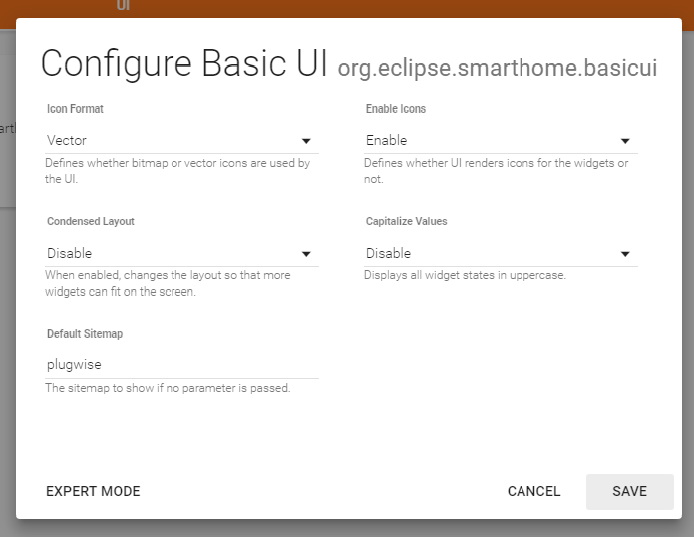
\includegraphics[width=0.5\textwidth]{Bilder/sitemapcfg}
	\caption{Sitemap-Konfiguration}
	\label{fig:sitemapcfg}
\end{figure}

\begin{figure}[H]
	\centering
	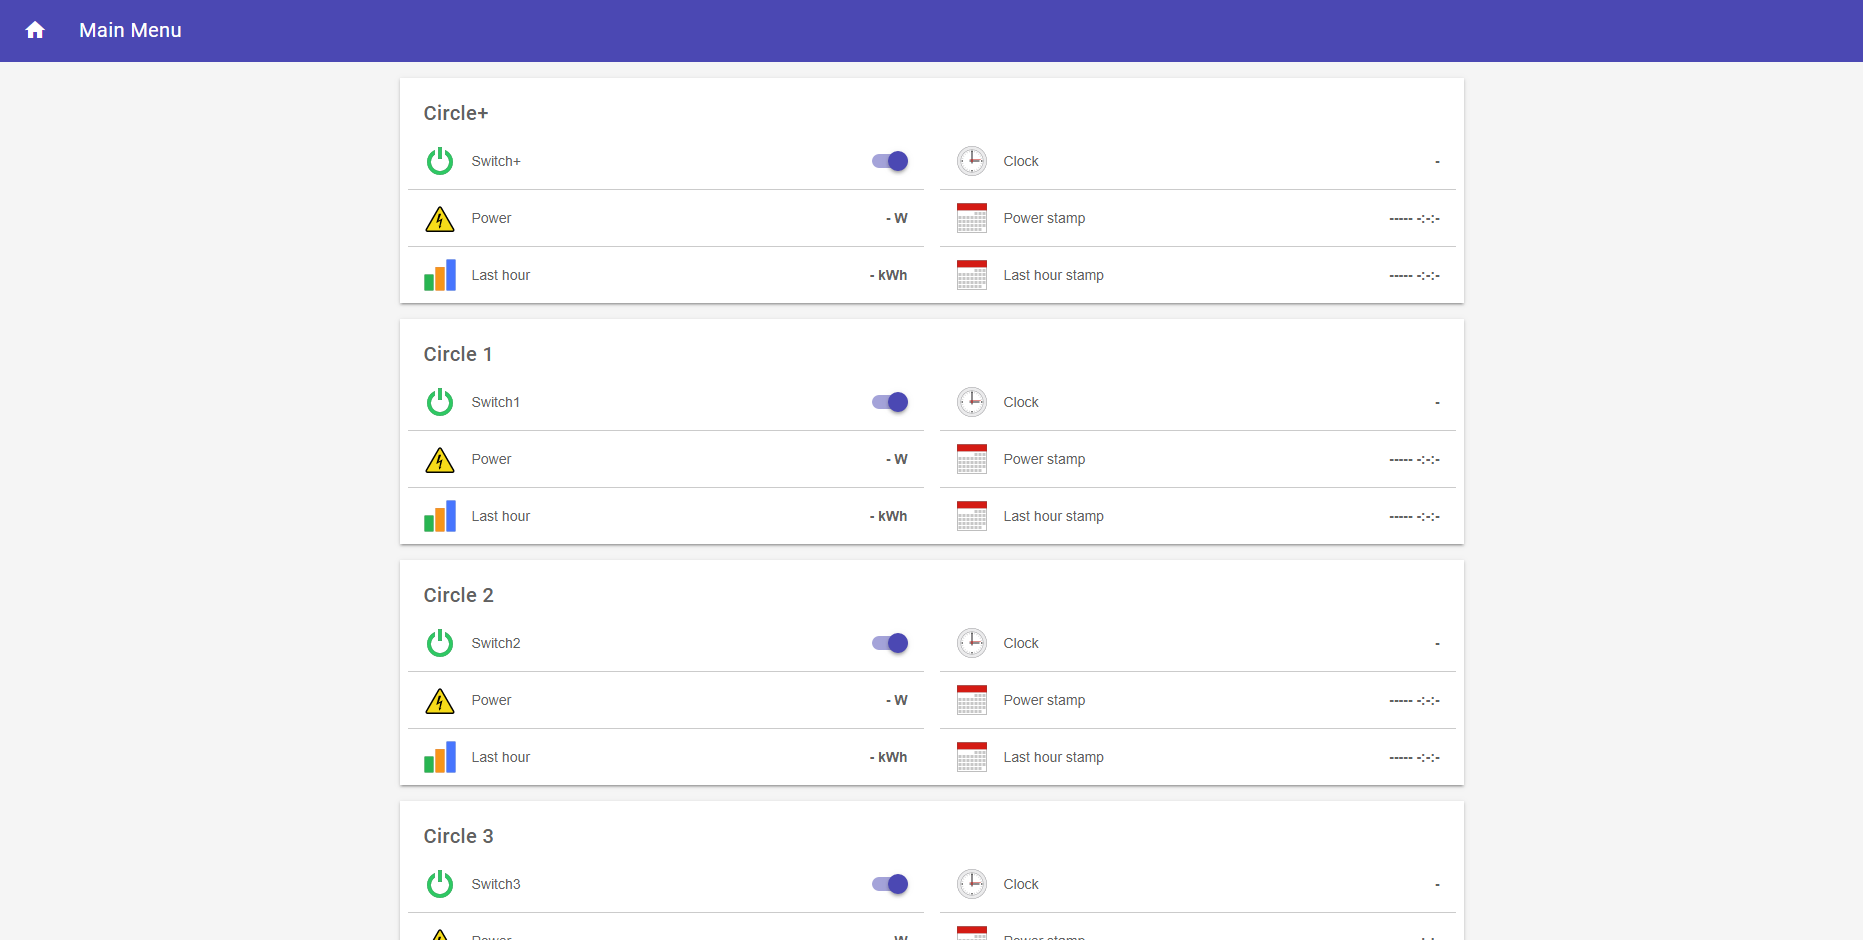
\includegraphics[width=1\textwidth]{Bilder/ohMain}
	\caption{Oberfläche im BasicUI}
	\label{fig:ohbasic}
\end{figure}

\newpage

\lstinputlisting[label=lst:pwSitemap, caption= Konfiguration der Benutzeroberfläche]{lst/pwSitemap.txt}

\textbf{Hinweis: }

Standardmäßig öffnet OpenHAB die Sitemap \textbf{default.sitemap}. Um auf die benutzerdefinierte Sitemap umzuschalten, muss deren Name (der in der ersten Zeile der Sitemap-Konfigurations-Datei definiert wird; \textbf{hier: } smarthome) im \textbf{Paper UI} unter '\textbf{Configuration}' $\rightarrow$  '\textbf{Services}' $\rightarrow$  '\textbf{Basic UI}' (oder andere Benutzeroberfläche) $\rightarrow$  '\textbf{Configure}'$\rightarrow$  '\textbf{Default Sitemap}' eingetragen werden (s. Abb. \ref{fig:sitemapcfg}). 

\newpage

\section{Präsenzerkennung}
\subsection{Bluetooth}
Zur Anwesenheitserkennung per Bluetooth kann der Ansatz gewählt werden, zunächst ein Skript zu erstellen, welches überprüft, ob ein bestimmtes Gerät vorhanden ist. Dieses Skript kann dann mit OpenHAB ausgeführt werden.

Einrichten von Bluetooth:
https://www.pi-supply.com/make/fix-raspberry-pi-3-bluetooth-issues/
\subsubsection{Vorbereitung}
\begin{itemize}
	\item \textbf{Bluetooth einrichten}
	\item \textbf{MAC-Adressen bestimmen}: Mit Hilfe \texttt{hcitool scan} lassen sich die MAC-Adressen aller Bluetooth-Geräte herausfinden, die sich gerade in der Umgebung des Pi befinden.
	\item \textbf{Bash-Skript} (hier \textbf{btSkript.sh}) zum Pingen bestimmter Bluetooth-Geräte erstellen (s. \autoref{lst:btBash}). Das Skript muss mit \texttt{chmod +x btSkript.sh} ausführbar gemacht werden. Durch \texttt{Pfad/btSkript.sh 1} bzw. \texttt{Pfad/btSkript.sh 2} kann die Funktionalität des Skripts geprüft werden. Mittels \texttt{chmod 777 btSkript.sh} wird die Ausführung der Datei für alle User, unter anderem auch OpenHAB, ermöglicht.
\end{itemize}


\lstinputlisting[label = lst:btBash, caption = Bash-Skript zur Präsenzerkennung mittels Bluetooth]{lst/bashBluetooth.txt}

\subsubsection{Einrichtung in OpenHAB}

Für die Ausführung des Skripts muss das \textbf{Exec Binding} installiert werden. Mit diesem können Kommandozeilen-Befehle ausgeführt werden. Hierfür muss ein \textbf{Thing} erstellt werden. Hierfür legt man unter \textbf{/etc/openhab2/things} eine Datei mit der Endung \textbf{.things} an, z.B. \textbf{btSkript.things}. In dieser wird jeder Befehl als Thing wie folgt definiert:
\begin{lstlisting}
Thing exec:command:bluetooth [command="sudo /home/pi/bt.sh 2", interval=10, timeout=5, autorun=false ]
\end{lstlisting}

Dadurch wird der Befehl \textbf{sudo /home/pi/bt.sh 2}, welcher überprüft, ob das Smartphone vorhanden ist, alle 10 Sekunden ausgeführt.\\
Für die Ausführung des Befehls muss jedoch noch zunächst ein \textbf{Item} erstellt werden. Hierzu wird unter \textbf{/etc/openhab/items} eine neue Datei, \textbf{anwesenheit.items}, angelegt. 
In diese trägt man die Zeile 
\begin{lstlisting}
String BT_Output "Anwesenheit [%s]" <light> {channel="exec:command:bluetooth:output"}
\end{lstlisting} ein. Dieses Item nimmt den Wert an, der durch das Ausführung des Skriptes zurückgegeben wir (also entweder "'ON"' oder "'OFF"'). "'<light>"' bezeichnet dabei das Icon, welches in der Benutzeroberfläche bei der Anwesenheit erscheint, in diesem Fall eine Glühbirne. \\


Für die Darstellung wird in der bereits beschriebenen Datei \textbf{smarthome.sitemap} der folgende Eintrag erstellt: 
\begin{lstlisting}
Text item=BT_Output label="Bluetooth [MAP(praesenz.map):%s]"
\end{lstlisting}
Außerdem muss zusätzlich das Binding \textbf{Map Transformation} (unter dem Reiter \textbf{Transformations}) installiert werden. Mit diesem können selbstdefinierte Werte, wie z.B. "'ON"' und "'OFF"', auf andere Werte bzw. Zeichenketten gemappt werden (z.B. Anwesend/Abwesend) , die dann von OpenHAB dargestellt werden. Für eine Transformation muss unter /etc/openhab2/transform eine Map-Datei (z.B. praesenz.map) erstellt werden, die folgende Form haben sollte:

\begin{lstlisting}
ON=Anwesend
OFF=Abwesend
undefined=unbekannt
\end{lstlisting}


https://klenzel.de/3328

\subsection{WLAN}
Für die Anwesenheitserkennung mit WLAN gibt es die Möglichkeit, das Network Binding zu installieren. Dieses listet alle Geräte als Things auf, die mit dem lokalen Netz verbunden sind. Nachteilig an dieser Methode ist, dass die IP-Adresse des Gerätes zur Anwesenheitserkennung genutzt wird und diese sich somit nicht ändern sollte.

\subsubsection{Einrichtung}
Sobald man das Network Binding installiert hat, kann in PaperUI unter Inbox auf verbundene Geräte überprüft werden. Hierzu klickt man auf das "'+"' und wählt im folgenden Menü Network Binding aus. Anschließend werden die IP-Adressen aller verbundenen Geräte aufgelistet. Mit einem Klick auf das Häkchen kann das gewünschte Gerät als Thing hinzugefügt werden. Nun erscheint das Gerät in Configuration unter Things. Mit einem Klick auf das Gerät erscheint folgendes Menü :
\begin{figure}[H]
	\centering
	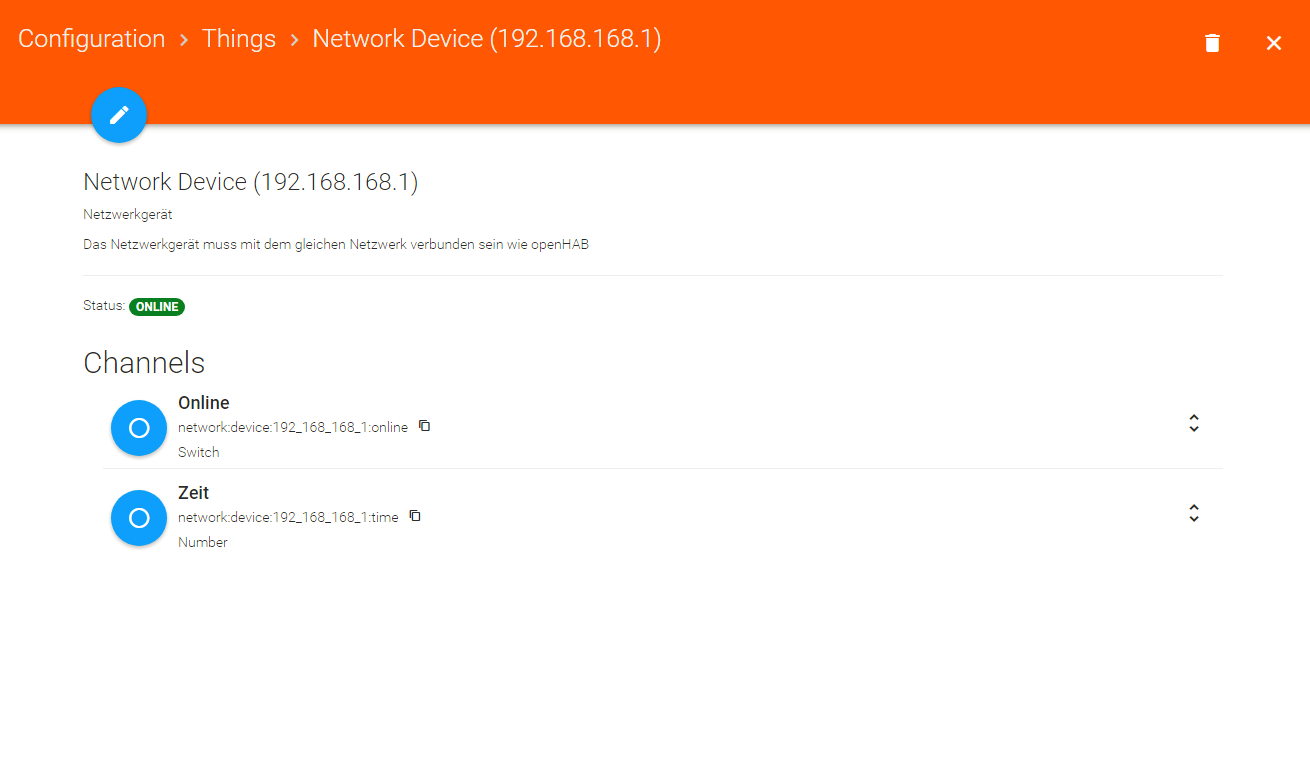
\includegraphics[width=0.9\textwidth]{Bilder/WLANthing.PNG}
	\caption{Menü des Gerätes}
	\label{fig:WLANthing}
\end{figure}

Hier kann bei Bedarf der Name geändert werden. Außerdem sieht man die verfügbaren Channels. Diese können einen bestimmten Wert einnehmen und mit einem Item verknüpft werden. Relevant ist in diesem Fall der Channel "'Online"', welcher anzeigt, ob das Gerät gerade mit dem Netzwerk verbunden ist. Mit einem Klick auf den Kreis erscheint ein Fenstermit einem Drop-Down-Menü, in dem alle verfügbaren Items aufgelistet sind, mit denen man den Channel verlinken kann. Außerdem kann ein neues Item erstellt werden, was in diesem Fall auch das Mittel der Wahl ist. 

\begin{figure}[H]
	\centering
	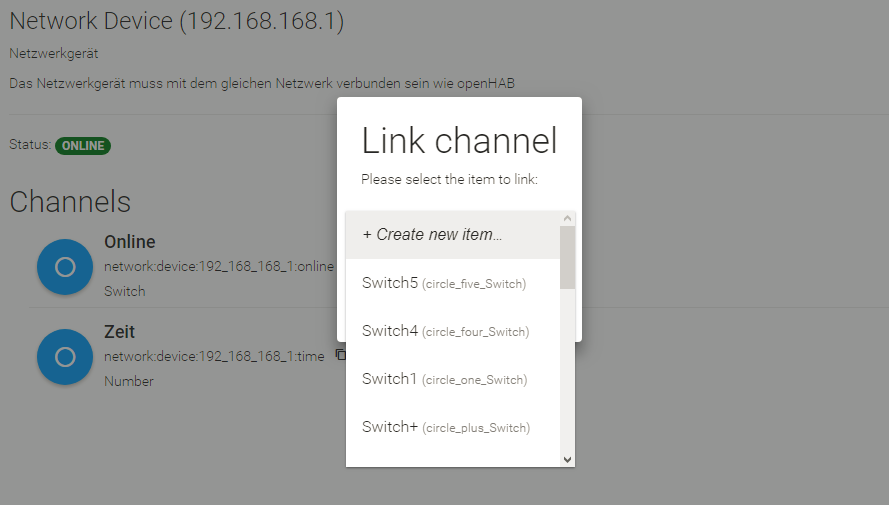
\includegraphics[width=0.9\textwidth]{Bilder/WLANchannel.PNG}
	\caption{Menü des Channels}
	\label{fig:WLANchannel}
\end{figure}

Damit gelangt man zum in \autoref{fig:linkChannel} gezeigten Menü. Hier kann man den Namen des Items ändern, diesen sollte man auch möglichst gut zuordnen können (z.B. Smartphone\_Status). Die weiteren Optionen werden so belassen.

\begin{figure}[H]
	\centering
	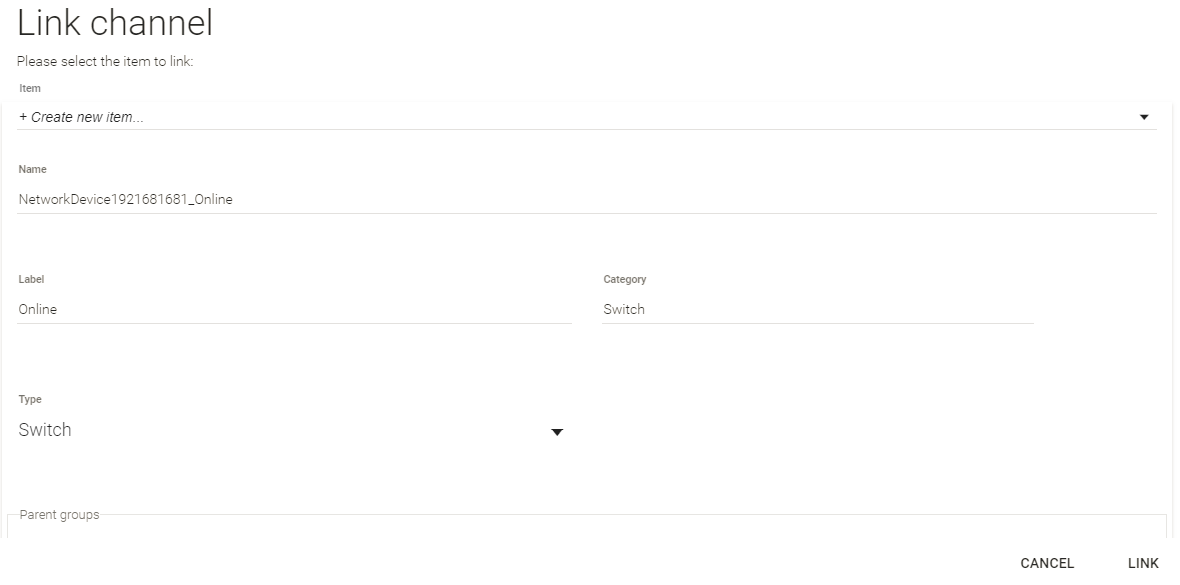
\includegraphics[width=0.9\textwidth]{Bilder/linkChannel.PNG}
	\caption{Link-Menü}
	\label{fig:linkChannel}
\end{figure}

Weiterhin muss das Item in anwesenheits.items eingefügt werden. Dies kann beispielsweise so aussehen:

\begin{lstlisting}
Switch smartphone "Smartphone" <light>
\end{lstlisting}

Für die Darstellung kann wie gewohnt ein Eintrag in smarthome.sitemap erstellt werden:
\begin{lstlisting}
Text item=smartphone label="Smartphone [MAP(praesenz.map):%s]" 
\end{lstlisting}

Auch hier wird das Mapping von "'ON"' zu "'Anwesend"' bzw. "'OFF"' zu "'Abwesend"' genutzt.

\paragraph{Gruppierung}
Damit die Benutzeroberfläche nicht zu unübersichtlich wird, wenn man mehrere Geräte/Methoden zur Anwesenheitserkennung nutzt, können die Geräte untereinander zu Gruppen zusammengefasst werden.

Binding: Network
Thing : IP-Adresse des Geräts
mit Item verbinden
Rules: Statusänderung
Gruppierung mit Gruppen

\subsection{RFID-Modul}

\subsubsection{Verbinden mit dem Raspberry Pi}

\begin{figure}[H]
	\centering
	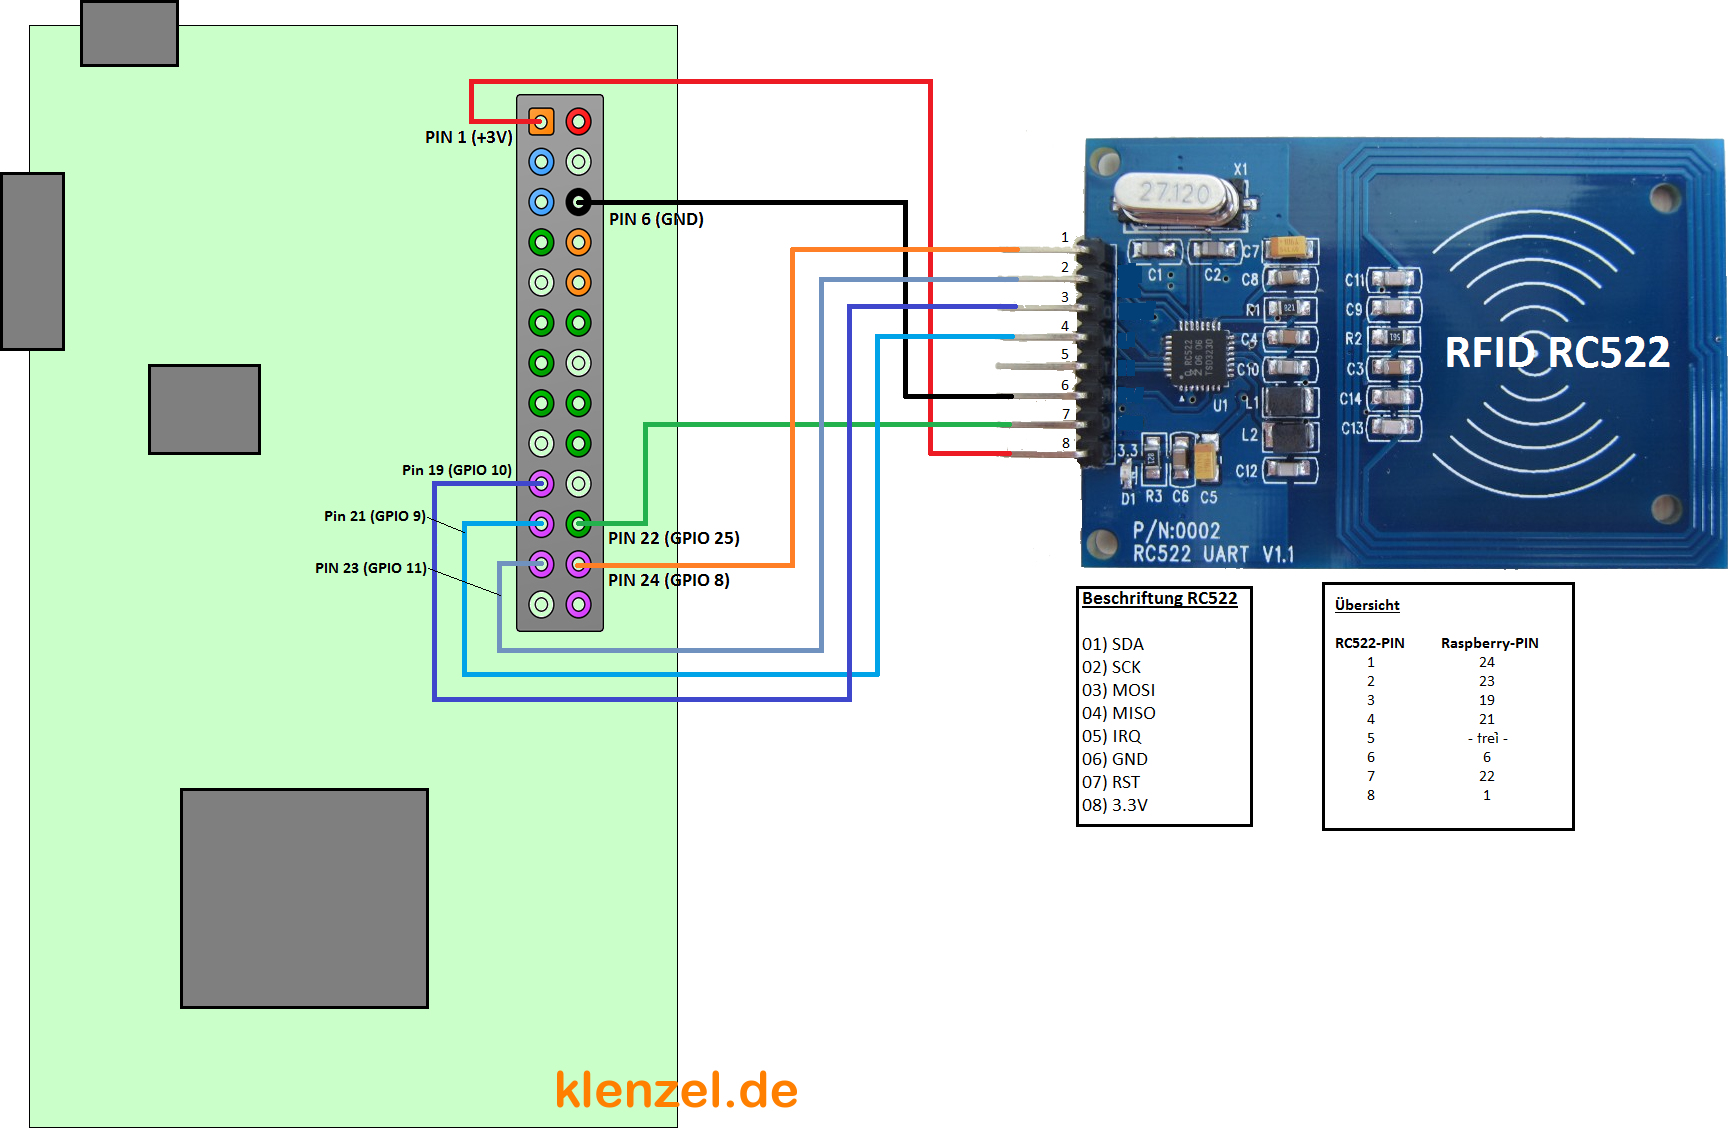
\includegraphics[width=0.9\textwidth]{Bilder/RFID.png}
	\caption{Verbinden des RFID-Moduls mit dem Raspberry Pi }
	\label{fig:RFID}
\end{figure}

Setup: https://tutorials-raspberrypi.de/raspberry-pi-rfid-rc522-tueroeffner-nfc/

\subsubsection{Python Skript}

\paragraph{State Machine}

\lstinputlisting[label=lst:stateMachine, caption = {Python-Skript mit State Machine zur Präsenzerkennung mit RFID-Modul}, language=Python]{lst/stateMachine.py}


\section{Graphische Darstellung der Daten mit LabVIEW}
Für die Darstellung der ausgelesenen Daten wird ein \textbf{LabVIEW\footnote{\textbf{LabVIEW}: \textbf{Lab}oratory \textbf{V}irtual \textbf{I}nstrument \textbf{E}ngineering \textbf{W}orkbench, ist ein graphisches Programmiersystem von \textbf{National Instruments}. Die Programmierung erfolgt nach dem Datenfluss-Modell in der graphischen Programmiersprache \textbf{G}.}-Programm} geschrieben.
Zur Kommunikation mit Datenbanken stellt das \textbf{LabVIEW Database Connectivity Toolkit} einige Programme bzw. Funktionen bereit. Diese nutzen \textbf{ODBC} um auf die Daten zuzugreifen. Das Programm bietet die Möglichkeit einzustellen, aus welchem Zeitraum die Datensätze ausgelesen werden sollen.

%Um die ausgelesenen Daten darzustellen, wird ein \textbf{LabVIEW}-Programm erstellt.
%...bla bla labview database connectivity toolkit. das kann odbc nutzen. mit select alle %datensätze zwischen a und b besorgen... sowas halt. mehr ins detail gehen lohnt sich dann, %wenn das programm mal fertig ist



% "Schaltung" einfügen
%Screenshot einfügen
\section{php}

\appendix
\chapter{Anhang}
\section{Einrichten einer statischen IP-Adresse}
Um dem Raspberry Pi eine statische IP-Adresse zuzuweisen, müssen in die Konfigurationsdatei \textbf{/etc/network/interfaces} folgende Zeilen hinzugefügt werden:

\begin{verbatim}
# Ethernet
auto eth0
allow-hotplug eth0
iface eth0 inet static
address 192.168.1.2
netmask 255.255.255.0
gateway 192.168.1.1
dns-nameservers 192.168.1.1
\end{verbatim}
Die entsprechenden Punkte müssen dabei gegebenenfalls an das eigene Netzwerk angepasst werden.\\
In \textbf{Raspbian Jessie} muss zudem der DHCP-Client deaktiviert werden (falls dieser sicher nicht gebraucht wird), da sonst diese Art der Konfiguration nicht funktioniert. Dies geschieht mit 

\begin{verbatim}
sudo service dhcpcd stop
sudo systemctl disable dhcpcd
\end{verbatim}

Falls man \textbf{nicht} über SSH verbunden ist, kann man entweder mit "'\texttt{sudo service networking restart}"' das \textbf{networking} oder das Interface \textbf{eth0} mittels "'\texttt{sudo ifdown eth0}"' und "'\texttt{sudo ifup eth0}"' neustarten.


\section{Serielle Schnittstelle zum Raspberry Pi}

Zur Nutzung der Schnittstelle muss diese zunächst im Konfigurationsmenü unter 'Advanced Options' eingeschaltet werden. Anschließend können die GPIO-Pins 4 und 5 als Tx bzw. Rx genutzt werden. Zum Testen der Funktionsfähigkeit wird die Software \texttt{minicom} genutzt. Durch den Befehl \texttt{sudo minicom -b 115200 -D /dev/ttyS0 -o} lässt sich die Schnittstelle öffnen. Pin 4 und Pin 5 werden mit einem Kabel verbunden und per \texttt{minicom} Zeichen gesendet. Diese erscheinen in der Konsole.



\section{FHEM-Modul für Plugwise-Steckdosen}
FHEM bietet ein internes Modul an, um die Steckdosen anzusprechen und zu konfigurieren. Um dieses zu benutzen, legt man ein neues device an (define myPlugwise Plugwise /dev/ttyUSB0). Dadurch wird der Stick definiert.


Die Abbildungen unten zeigen das FHEM-Menü und ausgelesene Daten (Energieverbrauch).\newline

\begin{figure}[H]
  \caption{FHEM Hauptseite}
  \centering
  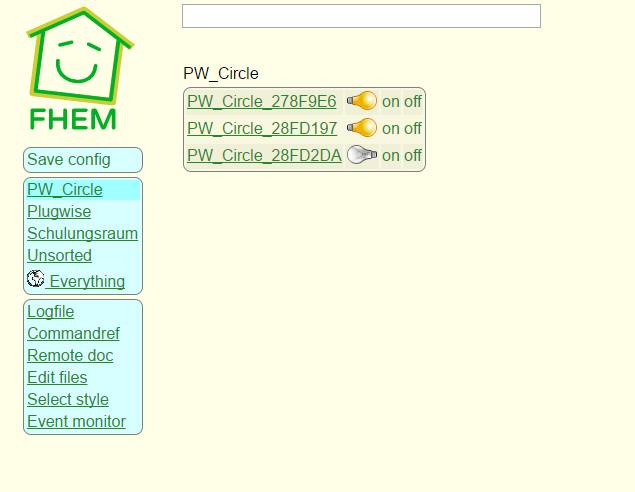
\includegraphics[width=6cm]{Home1}
\end{figure}

\begin{figure}[H]
  \caption{Konfigurationsmenü des Plugwise Sticks}
  \centering
  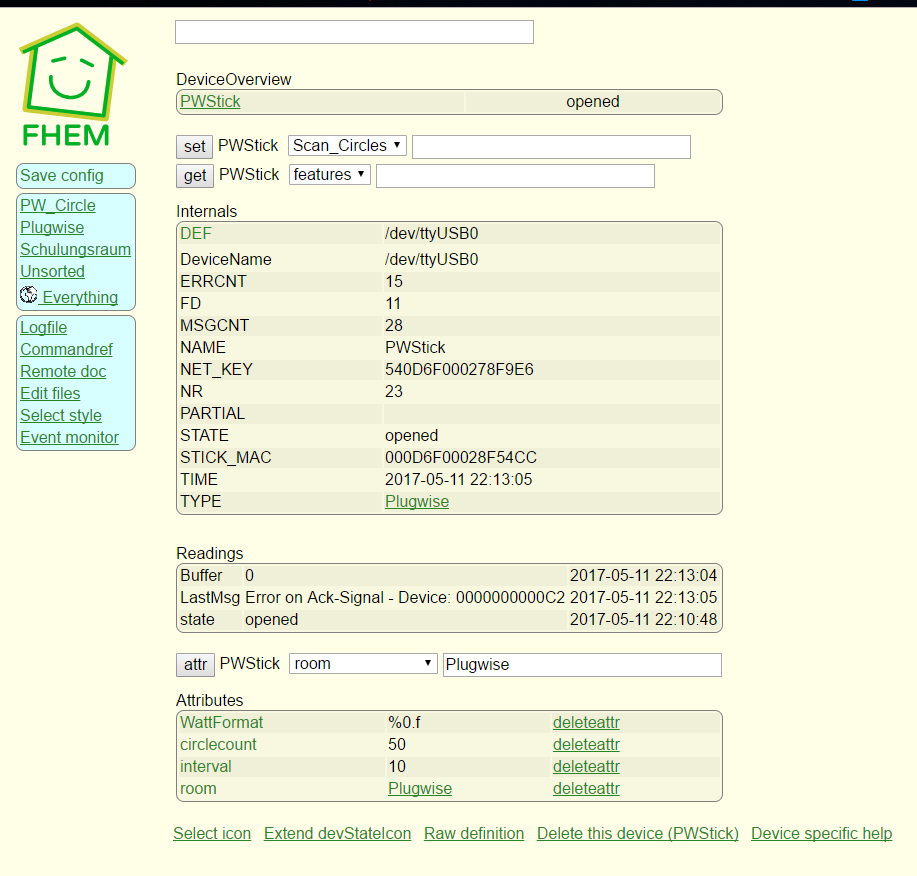
\includegraphics[width=6cm]{PWStick}
\end{figure}

\begin{figure}[H]
  \caption{Ausgelesener Energieverbrauch (Ausschnitt)}
  \centering
  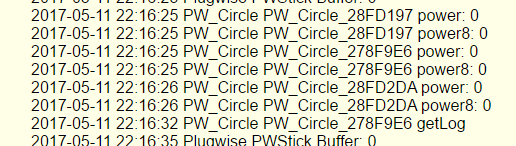
\includegraphics[width=0.5\textwidth]{FHEMPowerlogklein}
\end{figure}

\subparagraph{Probleme}\mbox{} \\
Damit die Circles überhaupt gefunden werden, muss versucht werden, parallel zu FHEM andersweitig die Steckdosen anzusprechen, z.B. mittels \texttt{plugwise-util}. Dabei findet FHEM nur einige der Steckdosen. Außerdem können nach einer Weile die Steckdosen nicht mehr gesteuert werden.\newline \newline





% ----------------------------------------------------------------------------

\begin{thebibliography}{99}
\bibitem{c1}https://de.wikipedia.org/wiki/OpenHAB (abgerufen am 22.07.2017)
\bibitem{c2}http://docs.openhab.org/installation/linux.html (abgerufen am 22.07.2017)
\bibitem{c3}http://docs.openhab.org/configuration/items.html
\bibitem{c4}http://docs.openhab.org/addons/bindings/plugwise1/readme.html\#pushed-state
\bibitem{c5}https://de.wikipedia.org/wiki/LabVIEW (abgerufen am 28.08.2017)
\bibitem{c6}https://wiki.ubuntuusers.de/mount/\#Optionen
\bibitem{c7}https://www.elektronik-kompendium.de/sites/raspberry-pi/2012181.htm
\end{thebibliography}

\end{document}
© 2019 GitHub, Inc.
Terms
Privacy
Security
Status
Help
Contact GitHub
Pricing
API
Training
Blog
About
